\subsubsection{Diagramma di Gantt}

I diagrammi di Gantt sono una rappresentazione su scala temporale dell'evoluzione del
progetto. Sono composti da varie barre orizzontali ognuna delle quali rappresenta una
attivit\'a che viene collocata sulla scala temporale in rappresentanza dell'attivi\'a stessa.
I diagrammi di Gantt hanno lo scopo di:
\begin{itemize}
\item definire cosa fare in una certa quantit\'a di tempo;
\item definire un riferimento per il controllo dell'avanzamento;
\item  definire degli eventi chiave dette milestones (fine di una fase, consegna).
\end{itemize}
Un diagramma di Gantt consente quindi la rappresentazione grafica di un calendario di
attivit\'a facilitando la pianificazione, il coordinamento e il tracciamento delle specifiche
attivit\'a dando una illustrazione dello stato di avanzamento del progetto. Per costruire
un diagramma di Gantt bisogna:
\begin{itemize}
\item  determinare le attivit\'a necessarie per concludere il progetto;
\item  stabilire il limite temporale del progetto;
\item  disegnare sul grafico il limite temporale stimato per ciascuna attivit\'a;
\item  verificare la presenza di discrepanze tra il tempo stimato e quello effettivamente
utilizzato.
\end{itemize}
Tramite i diagrammi di Gantt si identifica il percorso critico: alcune attivit\'a possono
partire solo dopo che altre sono finite, ognuna di queste attivit\'a viene detta critica e la
loro unione forma il percorso critico. \'E molto importante che le attivit\'a critiche non
subiscano slittamenti poich\'e questi si ripercuoterebbero, a cascata, su tutte le attivit\'a
critiche in attesa.

\subsubsection{Microsoft Project 2013}
Per la gestione e la pianificazione del progetto si \'e scelto di usare Project2013 essendo
un software dedicato al Project Management. Project2013 
crea automaticamente i diagrammi di Gantt una volta inserite le singole attivit\'a. Il software permette, inoltre, di modificare
le relazioni tra le attivit\'a e le date di inizio e fine nel caso le previsioni fatte non si
verifichino veritiere, o per l'insorgenza di problemi inaspettati. Questa funzionalit\'a
permette di mantenere il piano di progetto aggiornato con gli ultimi avvenimenti e d\'a
un idea del ritardo (o anticipo) acquisiti.

\subsubsection{Visione Globale del Progetto}
Viene presentata in questa sezione la visione generale del piano di progetto in modo da
dare una visione delle dipendenze tra le varie fasi, consentendo di comprendere:
\begin{itemize}
\item l'evoluzione temporale dell'intero progetto;
\item quanto pesa percentualmente ogni fase sia in senso economico che di tempo;
\item l'impiego delle varie risorse.
\end{itemize}
Di seguito sono presentate le immagini dei work package, ossia delle macro-attivit\'a in cui
\'e stato suddiviso il progetto, il diagramma di Gantt dell'intero progetto.
Il progetto risulta quindi avere un costo di \euro{}, a cui si dovranno andare a
sommare i costi di mantenimento e hosting del servizio.

\begin{figure}[H]
\begin{center}
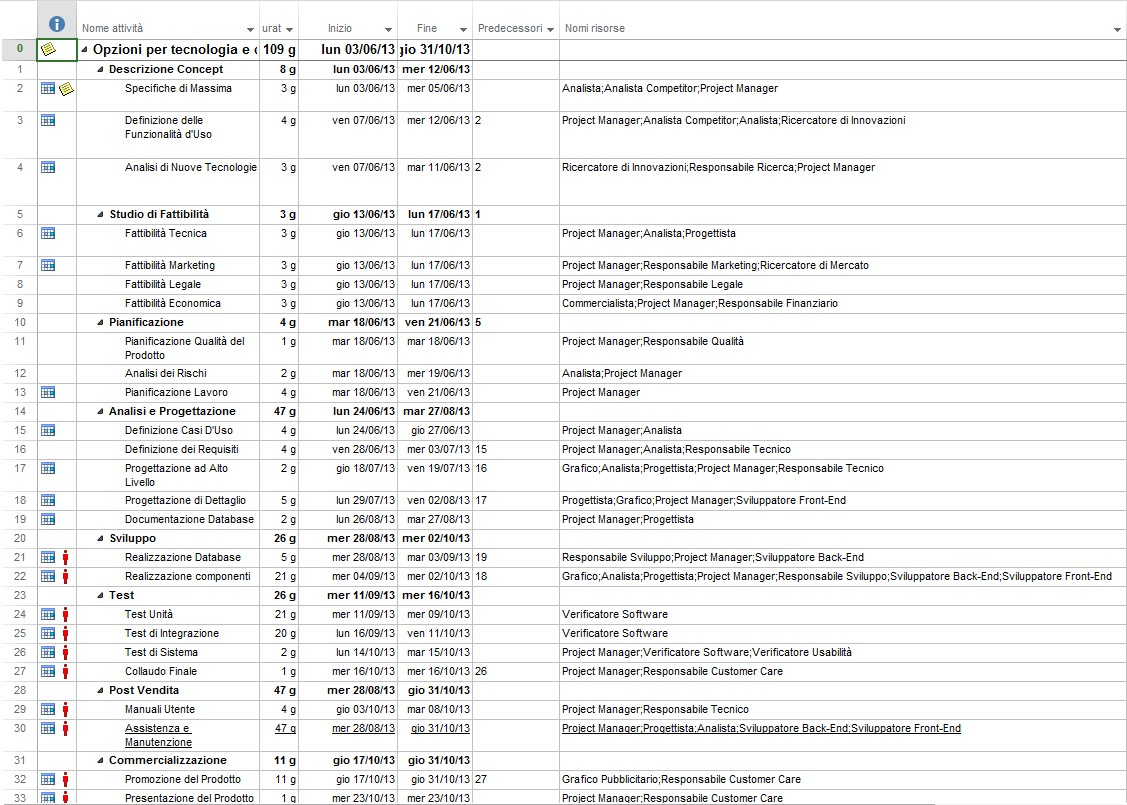
\includegraphics[width=1\textwidth]{img/Attivita.jpg}
\caption{Diagramma  Attivit\'a}
\label{fig:Diagramma Attivit\'a}
\end{center}
\end{figure}
\begin{figure}[H]
\begin{center}
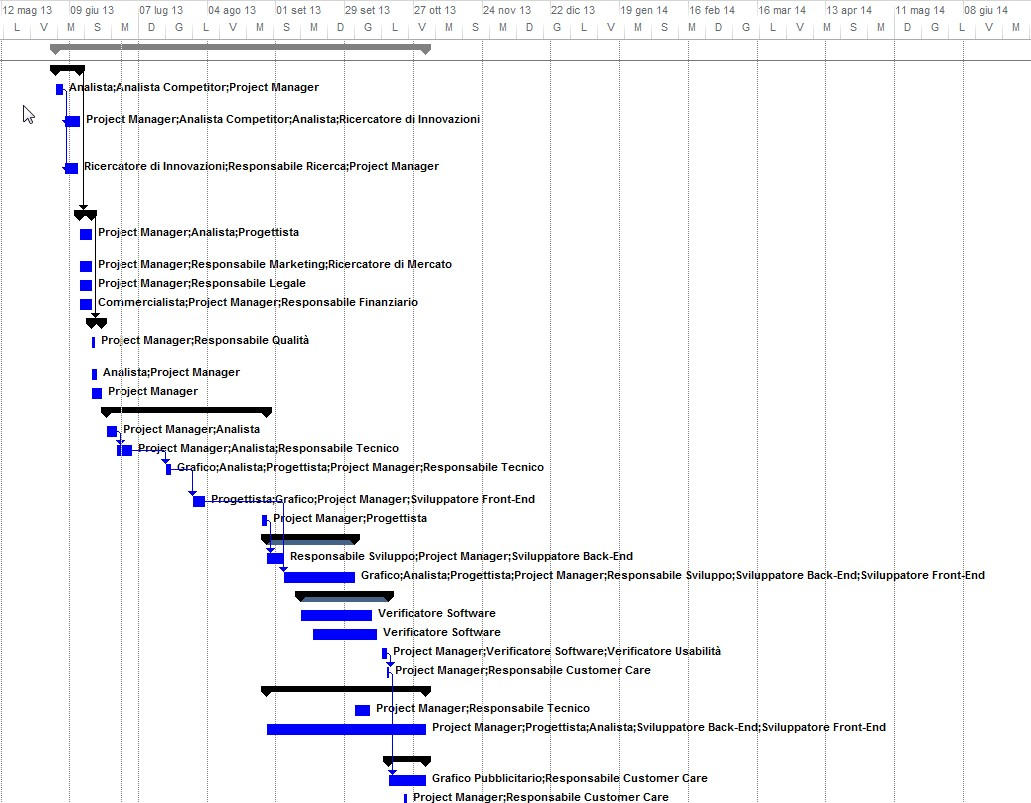
\includegraphics[width=1\textwidth]{img/Gantt.jpg}
\caption{Gantt Progetto}
\label{fig:Gantt Progetto}
\end{center}
\end{figure}
\newpage
\subsubsection{Gantt Milestone}

\begin{figure}[H]
\begin{center}
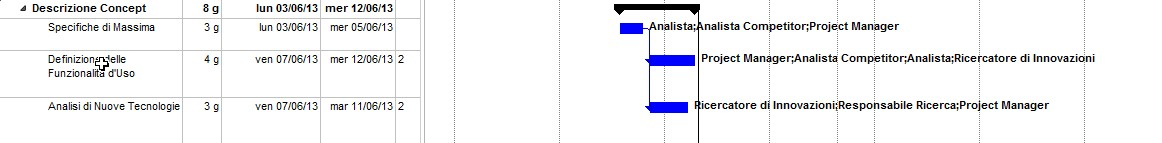
\includegraphics[width=1\textwidth]{img/G-A Concept.jpg}
\caption{Gantt Definizione Concept}
\label{fig:Gantt Definizione Concept}
\end{center}
\end{figure}

\begin{figure}[H]
\begin{center}
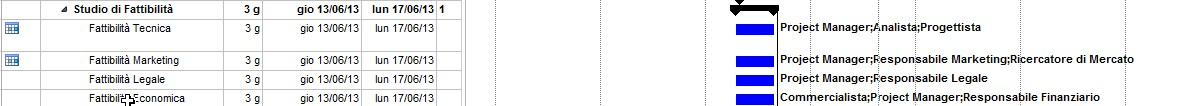
\includegraphics[width=1\textwidth]{img/G-A Fattibilita.jpg}
\caption{Gantt Studio di Fattibilit\'a}
\label{fig:Gantt Studio di Fattibilit\'a}
\end{center}
\end{figure}

\begin{figure}[H]
\begin{center}
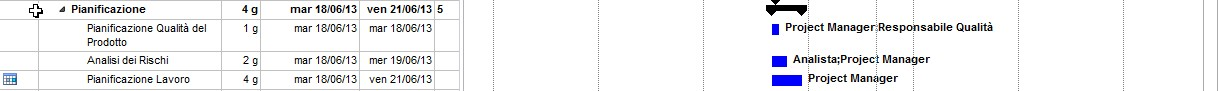
\includegraphics[width=1\textwidth]{img/G-A Pianificazione.jpg}
\caption{Gantt Pianificazione}
\label{fig:Gantt Pianificazione}
\end{center}
\end{figure}

\begin{figure}[H]
\begin{center}
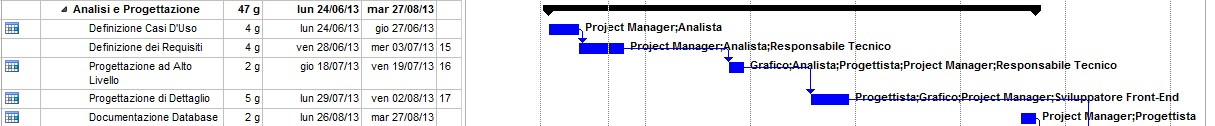
\includegraphics[width=1\textwidth]{img/G-A Analisi.jpg}
\caption{Gantt Analisi e Progettazione}
\label{fig:Gantt Analisi e Progettazione}
\end{center}
\end{figure}

\begin{figure}[H]
\begin{center}
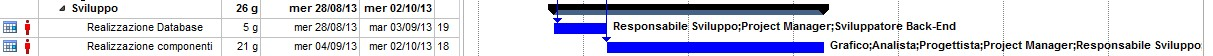
\includegraphics[width=1\textwidth]{img/G-A Sviluppo.jpg}
\caption{Gantt Sviluppo}
\label{fig:Gantt Sviluppo}
\end{center}
\end{figure}

\begin{figure}[H]
\begin{center}
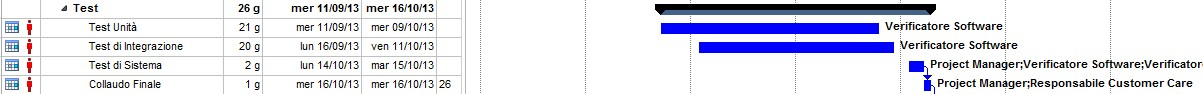
\includegraphics[width=1\textwidth]{img/G-A Test.jpg}
\caption{Gantt Test}
\label{fig:Gantt Test}
\end{center}
\end{figure}

\begin{figure}[H]
\begin{center}
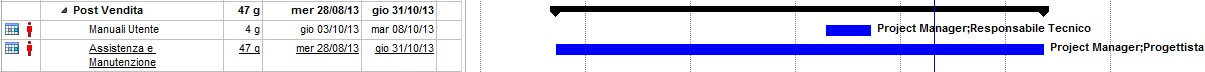
\includegraphics[width=1\textwidth]{img/G-A Vendita.jpg}
\caption{Gantt Vendita}
\label{fig:Gantt Vendita}
\end{center}
\end{figure}

\begin{figure}[H]
\begin{center}
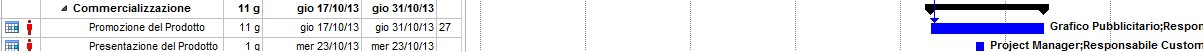
\includegraphics[width=1\textwidth]{img/G-A Commercializzazione.jpg}
\caption{Gantt Commercializzazione}
\label{fig:Gantt Commercializzazione}
\end{center}
\end{figure}